\section{DNABERT-2: Cải tiến với BPE và Multi-species Training}
\label{sec:dnabert2}

\subsection{Giới thiệu}

DNABERT-2 \cite{zhou2023dnabert} là thế hệ tiếp theo của DNABERT, giải quyết các hạn chế chính của người tiền nhiệm thông qua ba cải tiến quan trọng: Byte Pair Encoding tokenization, Attention with Linear Biases, và multi-species pre-training corpus.

\subsection{Byte Pair Encoding (BPE) Tokenization}

\subsubsection{Nguyên lý BPE}

BPE \cite{sennrich2015neural} là thuật toán compression được áp dụng cho tokenization. BPE xây dựng vocabulary bằng cách lặp lại merge các cặp symbols xuất hiện thường xuyên nhất:

\begin{enumerate}
    \item Bắt đầu với vocabulary chứa các nucleotides đơn: \{A, T, C, G\}
    \item Đếm tần suất của tất cả các cặp symbols liền kề
    \item Merge cặp xuất hiện nhiều nhất thành một token mới
    \item Lặp lại cho đến khi đạt vocabulary size mong muốn
\end{enumerate}

\textbf{Ví dụ:}
\begin{verbatim}
Iteration 1: "AT" xuất hiện nhiều nhất → merge thành "AT"
Iteration 2: "CG" xuất hiện nhiều nhất → merge thành "CG"
Iteration 3: "AT" + "CG" → merge thành "ATCG"
...
\end{verbatim}

DNABERT-2 sử dụng SentencePiece \cite{kudo2018sentencepiece} implementation của BPE với vocabulary size 4096.

\subsubsection{Ưu điểm của BPE}

\textbf{1. Loại bỏ information leakage:}

BPE tokens không overlap, do đó không có information leakage:
\begin{verbatim}
k-mer:  ATC TCG CGA GAT ATC TCG  (overlap)
BPE:    ATCG ATCG                 (no overlap)
\end{verbatim}

\textbf{2. Giảm độ dài chuỗi ~5 lần:}

Với vocabulary size 4096, BPE tạo ra tokens có độ dài trung bình ~5 nucleotides, giảm số tokens từ $L$ xuống $L/5$:

\begin{itemize}
    \item Giảm computational cost
    \item Giảm memory usage
    \item Tăng tốc training và inference
\end{itemize}

\textbf{3. Span prediction:}

MLM trên BPE tokens trở thành span prediction task - mô hình phải dự đoán cả độ dài và nội dung của span bị mask. Điều này đã được chứng minh làm tăng hiệu quả học \cite{raffel2020exploring}.

\begin{figure}[h]
    \centering
    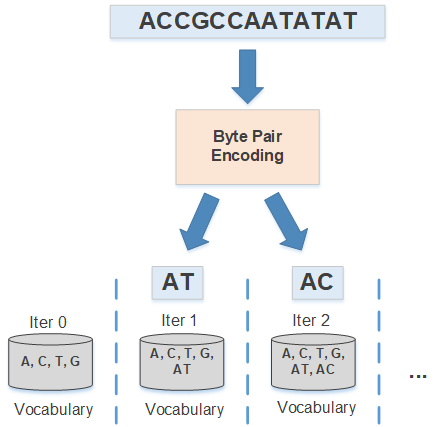
\includegraphics[width=0.6\linewidth]{imgs/bpe.png}
    \caption{Ví dụ về quá trình xây dựng vocabulary BPE (nguồn: paper DNABERT-2)}
    \label{fig:bpe}
\end{figure}

\subsection{Attention with Linear Biases (ALiBi)}

\subsubsection{Vấn đề với learned positional embeddings}

DNABERT sử dụng learned positional embeddings, bị giới hạn bởi maximum sequence length được định trước (512 tokens). Để xử lý chuỗi dài hơn cần retrain mô hình.

\subsubsection{ALiBi mechanism}

ALiBi \cite{press2021train} thay thế positional embeddings bằng bias được thêm vào attention scores:

\begin{equation}
\text{softmax}\left(\mathbf{q}_i \mathbf{K}^T + m \cdot [-(i-1), \ldots, -1, 0]\right)
\end{equation}

với $m$ là slope khác nhau cho mỗi attention head. ALiBi penalize attention weights dựa trên khoảng cách giữa query và key positions.

\subsubsection{Ưu điểm của ALiBi}

\begin{itemize}
    \item \textbf{Flexible sequence length}: Xử lý chuỗi có độ dài tùy ý mà không cần retrain
    \item \textbf{Better extrapolation}: Hiệu suất tốt trên chuỗi dài hơn training sequences
    \item \textbf{No additional parameters}: Không tăng số tham số mô hình
\end{itemize}

DNABERT-2 có thể xử lý chuỗi 10× ngắn hơn hoặc 15× dài hơn so với training sequences (trung bình ~700 bp) mà vẫn duy trì hiệu suất tốt.

\subsection{Multi-species Pre-training}

\subsubsection{Pre-training corpus}

DNABERT-2 được tiền huấn luyện trên corpus genome đa loài, bao gồm:
\begin{itemize}
    \item Genomes từ nhiều loài khác nhau (bacteria, archaea, viruses, eukaryotes)
    \item Tổng cộng hàng tỷ base pairs
    \item Đa dạng về GC content, codon usage, và genomic features
\end{itemize}

\subsubsection{Lợi ích}

\begin{itemize}
    \item \textbf{Better generalization}: Học các patterns bảo tồn qua các loài
    \item \textbf{Cross-species transfer}: Hiệu suất tốt trên các loài chưa thấy trong pre-training
    \item \textbf{Robust representations}: Ít bị overfitting vào đặc điểm của một loài cụ thể
\end{itemize}

Đặc biệt quan trọng cho phân loại phage, vì phage có đa dạng sinh học cao và nhiều phage chưa được nghiên cứu kỹ.

\subsection{Kiến trúc và Training}

\subsubsection{Model architecture}

DNABERT-2 sử dụng:
\begin{itemize}
    \item 12 transformer encoder layers
    \item 768 hidden dimensions
    \item 12 attention heads
    \item ~117M parameters (30\% nhiều hơn DNABERT)
\end{itemize}

\subsubsection{Flash Attention}

DNABERT-2 tích hợp Flash Attention \cite{dao2022flashattention} để:
\begin{itemize}
    \item Giảm memory consumption
    \item Tăng tốc training 3×
    \item Chỉ sử dụng 1/3 FLOPs so với DNABERT
\end{itemize}

\subsection{Hiệu suất}

\subsubsection{Genome Understanding Evaluation (GUE) benchmark}

DNABERT-2 đạt hiệu suất tương đương Nucleotide Transformer (2.5B parameters) trên GUE benchmark - 36 tasks trên 9 categories - trong khi:
\begin{itemize}
    \item Nhỏ hơn 21× về model size
    \item Nhanh hơn 92× về pre-training time
\end{itemize}

\subsubsection{Sequence length flexibility}

DNABERT-2 duy trì hiệu suất tốt trên:
\begin{itemize}
    \item Chuỗi ngắn: 70 bp (10× ngắn hơn training)
    \item Chuỗi dài: 10,000 bp (15× dài hơn training)
\end{itemize}

\subsection{Tại sao chọn DNABERT-2 cho PhaBERT-CNN}

DNABERT-2 là lựa chọn lý tưởng cho phân loại lối sống phage vì:

\begin{enumerate}
    \item \textbf{BPE tokenization}: Loại bỏ information leakage và hiệu quả tính toán
    \item \textbf{ALiBi}: Xử lý linh hoạt các contig có độ dài biến thiên (100-1800 bp)
    \item \textbf{Multi-species training}: Tổng quát hóa tốt cho phage đa dạng
    \item \textbf{Efficiency}: Model size và computational cost hợp lý
    \item \textbf{Strong baseline}: Hiệu suất tốt trên nhiều genomics tasks
\end{enumerate}

PhaBERT-CNN xây dựng trên nền tảng vững chắc này bằng cách thêm các lớp CNN đa tỷ lệ và attention pooling để trích xuất đặc trưng task-specific cho phân loại lối sống phage.
